\subsubsection{Scénario Cockburn}
\textbf{Cas d'utilisation: Payer par Télépéage}

\textbf{Acteur primaire:} Le conducteur

\textbf{Pré-condition: }  La borne est une borne télépéage ou voie mixte.
 
\textbf{Post-condition: } La transaction est acceptée, ou pas.

\textbf{Scénario primaire: } \\
    \textbf{1.} La borne détecte le badge télépéage\\
    \textbf{2.} La borne envoie la signature électronique du badge à l’ordinateur central de la société d’autoroute.\\
    \textbf{3.} L’ordinateur central de la société d’autoroute accepte la signature électronique du badge.\\
    \textbf{4.} La transaction est acceptée.

\textbf{Variantes:}\\
    \textbf{1a1.} La borne ne détecte pas le badge. \\
    \textbf{1a2.} Un technicien est appelé. Fin scénario.\\
    \textbf{3a1.} La signature du badge est invalide.\\
    \textbf{3a2.} La transaction échoue. Fin scénario.\\

\newpage
\subsubsection{Diagramme d'activité}
\begin{figure}[h]
    \centering
    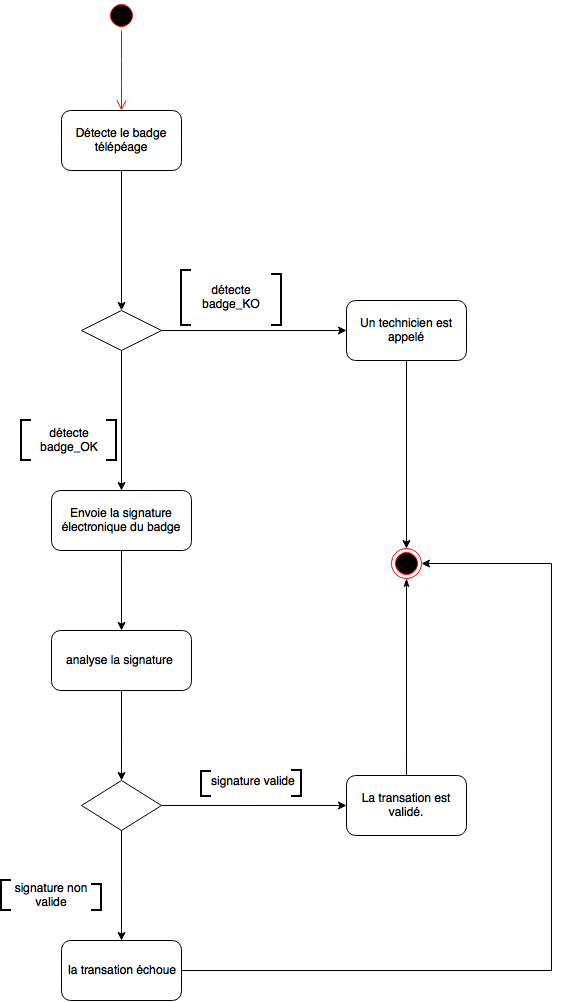
\includegraphics[scale=0.41]{02_Desenvolvimento/TD2/images/DATelepeage.png}
    \caption{Diagramme d'activité: Payer par Telépéage}
\end{figure}
\newpage
\subsubsection{Collaboration}
\begin{figure}[h]
    \centering
    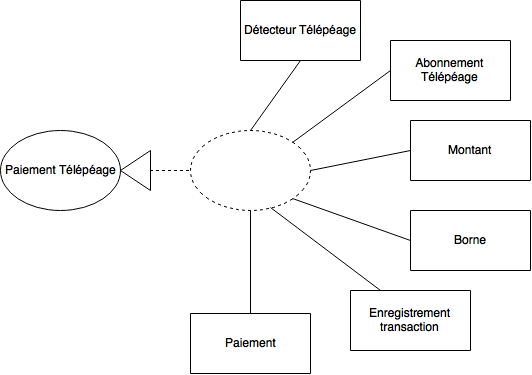
\includegraphics[scale=0.55]{02_Desenvolvimento/TD2/images/ColaTelepeage.png}
    \caption{Collaboration: Payer par Telépéage}
\end{figure}
\newpage
\subsubsection{Diagramme de sequence}
\begin{figure}[h]
    \centering
    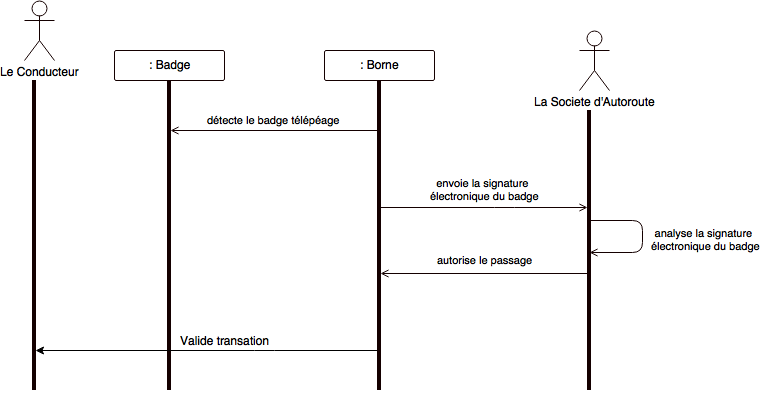
\includegraphics[scale=0.4]{02_Desenvolvimento/TD2/images/DS-PayerTelepeage.png}
    \caption{Diagramme de sequence: Payer par Telépéage à revisiter }
\end{figure}
\subsubsection{Diagramme de sequence}
\begin{figure}[h]
    \centering
    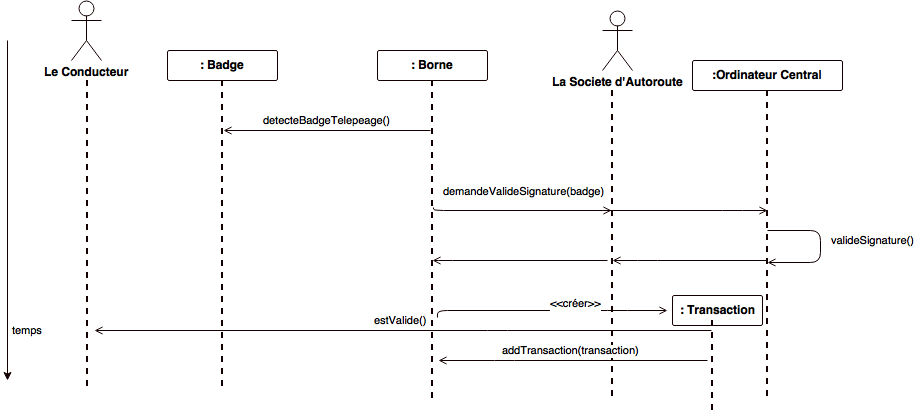
\includegraphics[scale=0.43]{02_Desenvolvimento/TD2/images/v2-DS-PayerTelepeage.png}
    \caption{Diagramme de sequence: Payer par Telépéage}
\end{figure}
